\documentclass[twoside,openright]{uva-bachelor-thesis}

%\usepackage[dutch]{babel}  % uncomment if you write in dutch
\usepackage{graphicx}
\usepackage{url}
\usepackage{mathtools}
\usepackage{amsmath}


% Title Page
\title{The Giving Game}
\author{Julian Ruger}
\supervisors{Peter Weijland (UvA)}
\signedby{}


\begin{document}
\maketitle

\begin{abstract}
This is the abstract. 
\end{abstract}

\tableofcontents

\chapter{Introduction}
In today's world money is the primary medium of exchange. Money is used to express the value of a transaction and is the major source of wealth. It's almost impossible to imagine an economy where no currency is used, even though it's more common than one may think. People often do not perceive giving as an economic transaction in the absence of a currency to express its value. However the contrary is true, giving is capable of establishing a whole independent economy. 

With today's technology giving is becoming an even more common occurrence. The internet is an important environment for communities where money is not used as a medium of exchange. File sharing and the availability of open-source software is a great example of such a giving economy. On a smaller scale giving is commonly used within communities of family and friends. Within this kind of communities giving away a good is not perceived as a direct loss, but instead it is expected that something will be given in return in the future. The value of transactions within such communities are determined by the relationship between the two participating parties of a transaction. People who have a better relationship with each other than with someone else value each other’s transactions more. 

The purpose of this thesis is to research the behaviour of people within an economy of giving under certain conditions. For example In real life people often seem to prefer to give to friends and family rather than to strangers. Thus they value a transaction with them more than with others. Under certain conditions people will assign a preference to a person or group of persons to who they will give to. 

\section{Contribution}
This thesis will research the behaviour of people within a giving economy from a game theory oriented perspective. A giving game designed by W.P. Weijland will be used to simulate an economy of giving. The goal of this thesis is to create a simulation program that can simulate a giving game of N agents and M goods. 
\\
\\
Chapter 2 will show the theoretical background of giving and the giving game. At the end of chapter 2 the research questions will be explained. Chapter 3 will describe the giving game used for this thesis and will show the simulation model that will be used to simulate the giving game. Chapter 4 will show the implementation of the giving game. The technical side of the simulation will be explained. Chapter 5 will describe the scenarios that will be used for the simulation. Chapter 6 will show the results of the scenarios from chapter 5. Chapter 7 discusses these results and answers the research questions. Lastly chapter 8 will suggest further research that can be accomplished with this thesis and the created simulation model.




\chapter{Theoretical background}
Giving occurs in multiple ways:
\begin{itemize}
  \item Giving can be giving something without getting something in return
  \item Giving can be giving something and getting something in return in the future.
  \item Giving can be a trade where something is giving and something is received.
\end{itemize}
When giving the value of the good is perceived differently by everyone. This means that when two goods are traded both goods do not necessarily need to be of the same value. To express the value of a transaction one may assume the existence of social credit. Social credit is an indication of the relationship between two people. Every individual keeps track of their own social credit balance with every other person and values a transaction in the light of this credit balance.

Based on this social credit people can have multiple reasons to give away something, but giving is almost always with the intention to get something in return. As shown in the article ‘Giving with Impure Altruism: Applications to Charity and Ricardian Equivalence’ even giving to charity is often not completely selfless. When giving out of kindness or to help someone else most people still get a good feeling. This feeling is called the ‘warm glow’. This shows that giving can still be with the intention to get something in return even if it seems to be out of kindness. This also shows that what is given in return does not have to be of the same value and that some people value giving to charity more than others, because of their perception of what they get in return.

In real life people often seem to prefer to give to friends and family rather than to strangers. Thus they value a transaction with them more than with others. Under certain conditions people will assign a preference to a person or group of persons to who they will give to.

The behaviour of people in an economy of giving can be a lot more complex than in an economy where money is used as a medium of exchange. With money it is easy to express a value of a transaction and almost everyone perceives this value the same. With giving this value is based upon multiple factors and can be different for every person.



\section{The economic model}
In the ‘ Kiyotaki-Wright Model’ an environment with three agents and three goods is simulated. Each agent produces one good and consumes another. This article shows the behaviour of the agents when they want to trade their good for the good they need to consume. This simulation used an economic environment without money, but only focused on scenarios where agents give away their good if they get a good in return which they can use. 
\\
\\
W.P. Weijland has created a similar model called ‘The Giving Game’, but instead focuses on more aspects of giving. A giving game is a game to simulate giving in real life. A giving game comes in many variants each of which aim to simulate certain aspects of real economic life. In this section the basic rules of a giving game are explained as well as the variant used for this thesis.
The following rules show the basics of a giving game:
\begin{itemize}
  \item In an environment of N agents an agent is randomly chosen to start with a good.
  \item Once an agent has the good the agent is meant to give it to someone else.
  \item Each time an agent receives the good the agent receives a credit point.
\end{itemize}

This thesis uses a variant of this giving game to simulate the behaviour of giving in real life under certain conditions.

\section{Mathematical background}
Every agent values the transaction of a certain good differently for each agent. This value of the transaction is called the yield. The value of a transaction is important for an agent to decide who to give to. For the calculations of the yield we first need to define some variables. Every agent has an account balance, the social credit, in relation to every other agent in the population. The account balance changes after every transactions based on the yield of the transactions. When a good is given away by P to Q the account balance is calculated as follows.\\
\\
\textit{new balance of P with Q = old balance of P with Q + yield} \\
\textit{new balance of Q with P = old balance of Q with P - yield} \\
\\
When P gives more the account balance of P gets higher. This can be interpreted as the more P gives to Q the higher the balance of P with Q thus the more P is ‘in the black’ with Q and the more Q is in debt with P. 
For the account balance between P and Q the following rule applies if P and Q agree on their mutual account balance.
\textit{Balance of P with Q = - (balance of Q with P)}
\\
\\
Every good also has a value and can be perceived differently by every agent. This is the nominal value and can be interpreted as an indication of how much someone wants this good. The nominal value of a good is set at the beginning of the giving game and does not change over time. The last variable we need to define is the like factor. The like factor is an indication of how much an agent likes another agent. The higher the like factor the more someone is liked.
For the model that is used for this thesis, these variables lead to the following calculations of the yield.
\\
\\
\textit{Y = a*x + b} \\
\textit{-1 $\le$ a $\le$ 0} \\
\textit{Y, b $\ge$ 0} \\
Here \textit{Y} is the yield, \textit{a} the like factor, \textit{X} is the account balance, and \textit{b} is the nominal value of a good. This function can be used to create a so called yield curve. Assuming we have a good \textit{G} that is given away by P to Q we get the following yield curve.
\\
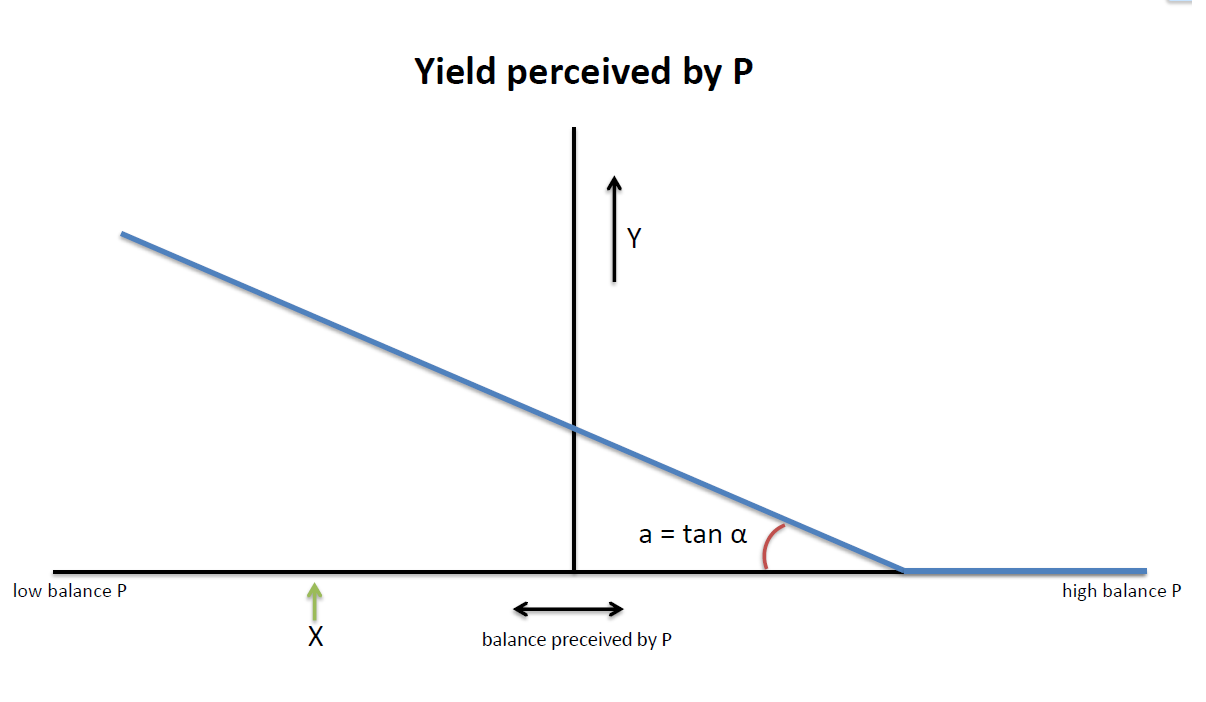
\includegraphics[scale=0.4]{YieldCurves/yieldcurve_P}
\\
From this yield curve it is clear that when the account balance of P with Q gets higher the yield gets lower.  When the yield gets lower the balance increases less, so for the next transaction the yield will also be less but will never reach zero.
The yield curve is not always a linear function. Different ways of calculating the yield can lead to different yield curves. This thesis makes use of a simplified version of the yield curve.

The yield will be important to determine who will receive a good next. If P would for example want to maximize its profit P would only want to give away a good to someone generating the highest yield. Agents who are in debt with P and are not likely to pay off their debt are of less value to P. It would be a bad investment if P would give to these agents.
\\
\\
The yield curve can either be used to predict the course of the transactions or to see an equilibrium arise. When an equilibrium arises the yield of a good between two agents switches between two values.  Both agents perceive the transactions with each other as the most valuable and will keep giving to each other. These agents have established a community with each other and this community will hold as long as the current condition do not change. 

\textbf{Image of yield curve with equilibrium here}

\section{Research questions}
As explained earlier, in real life people seem to prefer under certain conditions to give to 'friends' than to strangers. When people only give to a certain number of people the transactions will only take place within a small subgroup of the whole population. When this happens a community arises of people who prefer to give to each other. This is called the community effect. This has led to the following research question:
\\
\\
\textit{In a Giving Game simulation will transactions eventually take place within a limited subgroup of the entire population?}
\\
\\
Another possible behaviour that can be seen in an environment with an economy of giving is the stabilization of transactions. Even if no community effect emerges the transactions can still fall into a repeating sequence. The behaviour will be very predictable and the transactions are executed in a certain order. When the sequence of transactions is not random the transactions have stabilized. This has led to the second research question:
\\
\\
\textit{In a Giving Game simulation will we see a repeating sequence of transactions or will the transaction sequence look random?}


\chapter{Design}
For this thesis the giving environment consists of a fixed amount of agents and a fixed amount of goods. For every simulation the number of agents and number of goods can be changed, but during the simulation no agents or goods are added or removed.  Every agents keeps track of their own account balance and transaction values in relation to every other agent. The agents don’t know anything about each other, they operate completely independent.

There are two types of goods, ‘sustainable’ and ‘perishable’ goods. ‘Sustainable’ goods are goods that will exist for eternity. ‘Perishable’ goods are goods that perish after a certain amount of transactions. Every ‘perishable’ good has a producer. The producer is also an agent in the environment so the producer also participates in transactions of other goods. The producer reproduces its ‘perishable’ good after a certain amount of time the good has perished. The value of a good is valued differently by each agent, but this value does not change during the simulation. For the experiments in this thesis the agents are not able to hold on to a good for a certain amount of time. This is a variant which can be used in further research. Holding on to a good will be explained further in the last chapter. At the start of the giving game the goods can either be divided randomly over the agents or are divided by hand. The agents who start with the perishable goods are assigned to be the producers.

The transactions can be executed in two different ways. The transactions can be executed one by one which is a more game theory based approach. A more realistic approach is that the transactions are executed simultaneously, this way agents don’t have to wait for each other before they can give away their good. Both types are used in the experiments.

The emergence of a community effect is determined by the amount of transactions each agent is part of. When more than one good is used in the environment there can emerge multiple communities. That is why every good is looked at independently. Every agent keeps track of their own transactions and how much they have traded each good. If for example two agents hold 100 percent of the transactions of good A and two other agents hold 100 percent of the transactions of good B then two separate communities of size two have emerged. There can be concluded that the community effect exists for this scenario. If this time two agents hold 50 percent of the transactions of good A and good B and two other agents also hold 50 percent of the transactions of good A and good B than this means that one community has emerged with a size of four. There can also be concluded that a community effect exist in this scenario.  A community effect can exists as long as the size of the subgroup is smaller than the total amount of agents in the environment and 100 percent of the transactions of one or more goods takes place inside this subgroup. This means that even if an agents holds a smaller percentage of the transactions this agent can still be part of the community as long as the previous stated rules apply.

The stabilization of the transactions in the environment can be determined by predicting future transactions. If multiple transactions in a row can be predicted or if a pattern is clearly visible then one may conclude that the transactions have stabilized. The emergence of a community does not mean that the transactions are executed in a repeating sequence. Even in a community the transactions can be executed randomly.


\section{Paramaters}
The following parameters will be used in the environment of the giving game for the experiments.

\begin{description}
  \item[N:] The number of agents used in the simulation
  \item[M:] The number of goods used in the simulation
  \item[Perish period:] The perish period is the amount of transactions it takes before a good perishes. For sustainable goods the perish period is 0, because sustainable goods exist forever. For perishable goods the perish period is greater than 0. For example, when a good has a perish period of 3 then this good can be given away 3 times before it perishes. The perish period is a natural number greater than or equal to 0.
  \item[Production delay:] The production delay is the time between the perish of a good and its reproduction. The time until the production is decreased by one after every iteration over all agents who are currently holding a good. The production delay is a natural number greater than or equal to 0.
  \item[Nominal value:] The nominal value is an indication of how much a good is worth. The nominal value does not change during the giving game. Every agent perceives the nominal value of a good differently. Agent P could value good G more than agent Q for example. The nominal value is a natural number greater than or equal to 0.
  \item[Like factor:] The like factor is a real number between -1 and 0 which defines how much agent P likes agent Q. The higer the number the more P likes Q and the more likely it is that P will give to Q. The like factor does not change during the giving game. 
  \item[Selection rule:] The selection rule is an algorithm that decides/calculates the next agent(s) to receive a good.

\end{description}

\section{Selection rules}
For every transaction the selection rule decides which agent will receive a good. This decision is based on different parameters of the giving game. These selection rules simulate  multiple real world scenarios for example: choosing the agent based on maximizing the profit (goodwill rule).

\subsection{Random rule}
The random rule is the most basic rule for the giving game. The agent who will receive the good during the transaction is chosen randomly. The random rule simulates an environment where the agents do not care about the value of the goods and do not care about who will receive the goods. The \textit{like factor} is therefore 0 for every agent pair. This rule is mostly used to see if the giving game enviroment behaves as it should.

\subsection{Balance rule}
A more advanced selection rule is the balance rule. The agent who will receive the good during the transaction is selected based on the balance between the giving agent P and the receiving agent Q. Agent P chooses agent Q if P has the highest balance with Q. If P has the same highest balance with multiple agents then the receiving agent is chosen randomly between these agents. The balance rule simulates an environment where each agent only gives to the agent from who they have received the most. Agent P tries to maximize the number of goods he receives. The balance in this case can be calculated as follows: 
\\
\\
\textit{Balance of P with Q = Number of goods received from Q – Number of goods given to Q} \\
This calculation of the balance is different from the calculation of the balance for the yield curve, but the following rule still applies:\\
\textit{Balance of P with Q = - (balance of Q with P)}

\subsection{Goodwill rule}
The goodwill rule is a more realistic rule. The agent is chosen based on the value of the transaction (the yield) between P and Q perceived by P. Only the agent where the yield is the highest is chosen as the receiving agent. If multiple agent pairs have the same yield the receiving agent is chosen randomly between these agents. Every time P gives good G to Q the value of the transaction of good G (the yield) decreases. As long as Q does not give good G to P, P loses interest in giving good G to Q. Eventually P will stop giving to Q, because P does not expect that Q will ever pay of his debt. The like factor as explained earlier defines how many transactions P can tolerate without getting anything in return from Q. For the goodwill rule the like factor can be set by the user or can be created randomly. The goodwill rule simulates an environment where every agent tries to maximize its profit. Agents who are in debt will less likely receive a good, they are not worth investing in.
This leads to yield curves that look like this: \\
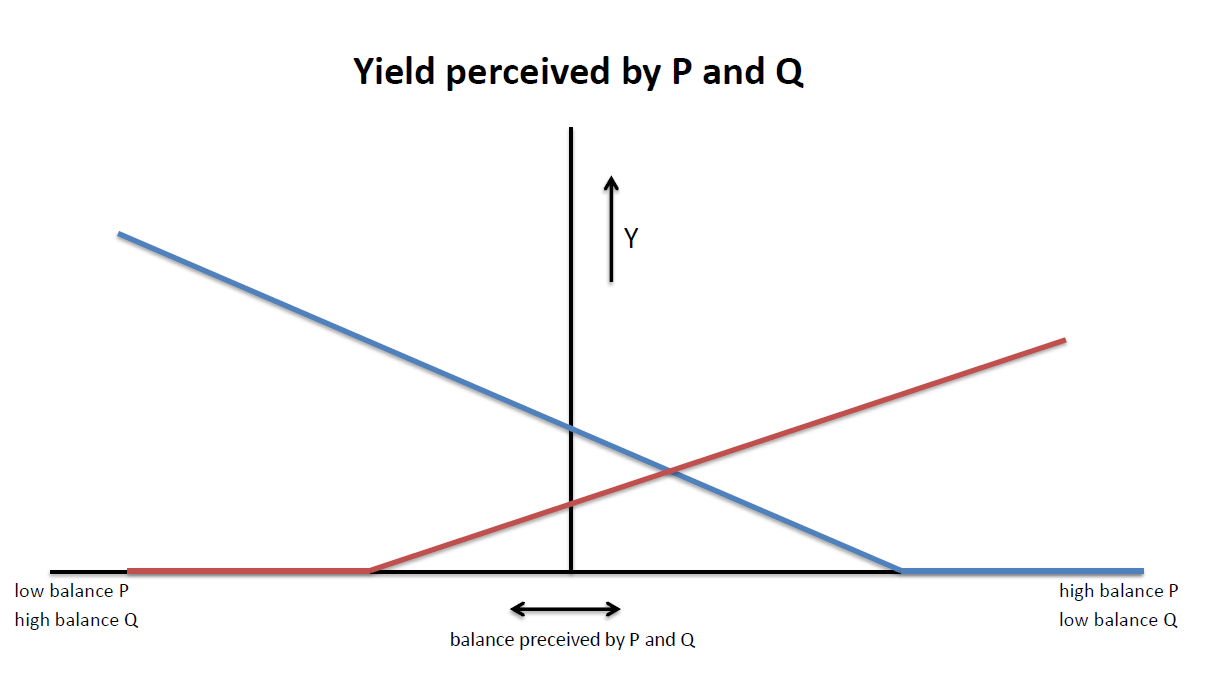
\includegraphics[scale=0.4]{YieldCurves/yieldcurve_PQ} \\
The steeper the slope for YP the less tolerant P is. In this case the balance is calculated as explained before.
\\
\\
The expectation to receive something in return of a gift actually transfoms that gift into an investment (with a certain likelihood to receive any gains in the future). The goodwill rule can be seen as a representation of an environment where people invest and all agents try to maximize profit they can get from such investment. A bad investment is looked down upon and in the future an investment in the same person will most likely not happen.

\section{Simulation model}
For the previously explained giving game a simulator will be created that can simulate different scenarios using the parameters and selection rules. The following flow chart shows the actions that are executed to simulate the giving game.

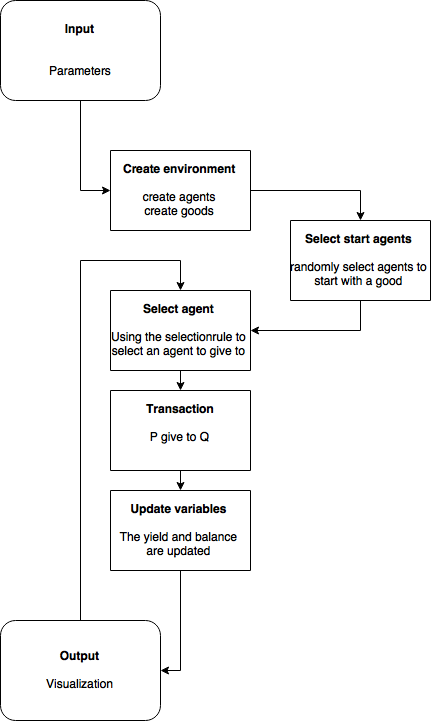
\includegraphics[scale=0.6]{FlowChart/FlowChart}

The technical side of the simulator will be explained in the next chapter. 

\chapter{Implementation}
\textbf{Work in progres!}
In this chapter the implementation of the simulator that will be used to simulate different scenarios for the giving game will be discussed. The simulation program is able to execute multiple tasks. The simulation program is able to accept different user input to simualte multiple scenarios. The simulation program provides a visualization of the data that is produced during the simulation and a visualization of the course of the transactions. The whole simulation program is created with Python and uses multiple Python packages and frameworks. The simulation program can be run on a desktop with any operating system as long as the required Python packes and frameworks are installed. 

\section{Back-end}
The back end consists multiple compononents which together create an environment that simulates an giving economy where agents give and receive goods. This section will explain these components briefly and how they work together. For a more detailed description of the back end the full documentation can be found in appendix A.

\subsection{Agents}
Every agent is defined by the \textit{Agent} class. Every agent can be identified by an \textit{ID}. This \textit{ID} is an integer number greater than or equal to 0. Every agent keeps track of their own account balance, yield values, like factors and nominal values. The \textit{Agent} class is able to hold this data in the form of a Python list. The ID of every agent is used for these data lists to find the corresponding information about that agent.

\subsection{Goods}
Every good is defined by the Good class.  Every good can be identified by an \textit{ID}. This \textit{ID} is an integer number greater than or equal to 0. This \textit{ID} can be used by the textit{Agent} class as an index for the python lists that hold information about this good.

\subsection{Selection rules}

\subsubsection{Random rule}

\subsubsection{Balance rule}

\subsubsection{Goodwill rule}

\subsection{Environment}

\subsection{Simulation}
The simulation is run by first creating the environment. The environment is created by first creating the Agents and the Goods. After the goods have been created the agents are notified, their perception of the nominal values of these goods and the yield values for the first transactions are updated. The goods are either randomly assigned to the agents or chosen by the user.


\section{Front-end}
The front end provides the interface between the user and the back end. With this interface the user is able to put data into the simulation to simulate different scenarios. The interface is able to visualize the responses of the back end to analyse the resulting data during the simulation. For the explanation of the use of the interface the use should consult the user manual which can be found in appendix B.

\subsubsection{Input}
The user is able to input the following parameters:

\begin{description}
  \item[N:] 
  \item[M:] 
  \item[Perish period:] 
  \item[Production delay:]
 \item[Selection rule:] 
  \item[Nominal value:] The user is able to choose if every agent perceives the value of a good differently or not. If the user wants to have a different value of the good for every agent the user can add a xslx file with the nominal values as follows:
  \item[Like factor:] The user is able to choose between setting like factors by hand or to randomly create the like factors. If the user wants to add predefined likefactors the user can add a xslx file with the like factors as follows:
 \item[Balance:] The user is able to set the balance at the start of the simulation at 0 or to add different balances for every agent.
\end{description}
During the simulation the user should be able to adjust the following variables:

\begin{description}
  \item[Subgroup size:] 
  \item[Reset community percentage:] 

\end{description}
\subsubsection{Output}
The output data is visualized so that the user is able to analyse and get results without doing any calculations. The simulator is able to do most of the work.

The simulator is able to give the following output:
\begin{itemize}
  \item Show the amount of goods given and received for each agent in a bar plot.
  \item Show the yield curve between every agent pair.
  \item Show the amount of transactions
  \item Show the visualization of the course of the transactions with a color indication for any emerging subgroups.
  \item Show percentages of how many times a certain good has been traded by an agent.
  \item Show every transaction, producting and delay in production.
  \item Show the community percentage (How many transactions take place in a subgroup with the current set size.)
\end{itemize}

All the data can be saved and used in the future for another simulation.


\chapter{Scenarios}
For every selection rule multiple scenarios have been created. This chapter will explain the scenarios used in the experiments. For every scenario 99 agents will be used. 99 agents is large enough to have as much variety in the parameters as possible but is still be able to clearly see any changes in the visualisation.  

\section{Basic Scenarios}
For every selection rule the behaviour is tested in the most basic environment. These scenarios will be used to see if the simulation behaves as it should.
\subsubsection{Basic scenario 1, sustainable (BS\_S):}
Parameters:
\begin{itemize}
\item	99 agents
\item	1 sustainable good with a nominal value of 1, perish time of 0, perish delay of 0
\end{itemize}
\subsubsection{Basic scenario 2, perishable (BS\_P):}
Parameters:
\begin{itemize}
\item	99 agents
\item	1 perishable good with a nominal value of 1, perish time of 1, perish delay of 1
\end{itemize}
In case of the goodwill rule where the like factor is used for the selection of an agent the like factor is set to -1 for every agent. In the most basic environment every agent is equal and has no specific relations with other agents.

\section{Random rule}
The following scenarios are  used to see if the agents behave as predicted with the random rule.  Any irregularities in the behaviour will be analysed and can be used in decisions for further experiments. The nominal value does not have to be set, because the nominal values of the goods are not used in the selection of an agent.
\subsubsection{Scenario 1, sustainable (RR\_S):}
Parameters:
\begin{itemize}
\item	99 agents
\item	3 sustainable goods
\end{itemize}
\subsubsection{Scenario 2, perishable (RR\_P):}
Parameters:
\begin{itemize}
\item	99 agents
\item	3 perishable goods with a perish time of [1,2,3], perish delay of [1,2,3]
\end{itemize}
The number of goods is not a fixed number, during the experiments the number of goods will differ to see if this affects the results.

\subsubsection{Hypothesis}
It is expected that no community effect will arise, neither will the simulation stabilize even though a machine is pseudorandom. The transactions will eventually be equally distributed over all the agents. For perishable goods this distribution will be in favour of the producers, because they will be able to give away their good more than others.

\section{Balance rule}
The scenarios for the balance rule will be used to see how people will behave when they care about how many goods they give and receive but do not have any relationship with other agents. The nominal value does not have to be set, because the nominal values of the goods are not used in the selection of an agent.
\subsubsection{Scenario 1, sustainable (BR\_S):}
Parameters:
\begin{itemize}
\item	100 agents
\item	3 sustainable goods
\end{itemize}
\subsubsection{Scenario 2, perishable (BR\_P):}
Parameters:
\begin{itemize}
\item	100 agents
\item	3 perishable goods with a perish time of [1,2,3], perish delay of [1,2,3]
\end{itemize}
The amount of goods is not a fixed amount, during the experiments the amount of goods will differ to see if this affects the results.

\subsubsection{Hypothesis}
The expectations are that a community effect will arise with a subgroup consisting of a few agents. The size of this subgroup is based on the type of goods and the amount of goods. All sustainable goods will eventually be traded only between two agents, because these two agents have the highest balance with each other. Every perishable good has a producer, these producers will also be part of a subgroup. If these producers only give each other their goods then the subgroup size will be as large as the amount of producers. If the producers each give to another agent then multiple subgroups will arise with a size of two. It is expected that the maximum size of a subgroup will be the number of producers plus one non-producer who trades with the producers.

\section{Goodwill rule}
For the goodwill rule all parameters can affect the results. The following parameters define the scenarios.
\subsubsection{Like factors}
\begin{description}
\item[L1]	1/3 of the population has a like factor of -1, 1/3 of the population has a like factor of -0.5 and 1/3 of the population has a like factor of -0.1. This means that every agent has a different relationship with every third of the population. These three groups have been chosen in order to better observe the difference in behaviour.
\item[L2]	47 agents have a like factor of -1, 47 agents has a like factor of -0.5 and 5 of the agents have a like factor of -0.1. This means that only a small group of agents is liked by all other agents.
\end{description}
\subsubsection{Balances}
\begin{description}
\item[B1]	At the start of the simulation all account balances are set to 0.
\item[B2]	At the start of the simulation all account balances are randomly set. The account balance for every agent will be a real number between -1 and 1, because the minimal nominal value of a good will be 1. If the account balance would be less than -1 or greater than 1 then the yield could fall below 0, which should not be possible according to the defined yield curve for this thesis.
\end{description}
\subsubsection{Nominal values}
\begin{description}
\item[N1]	The nominal values of every good are the same for every agent.
\item[N2]	Every third of the agents perceives the nominal values of all goods differently. Just like the like factors, the population is divided into 3 groups, where every group perceives the value of the goods differently. The first group perceives the nominal value of the good as 1, the second group as 2 and the third group as 3. For every additional good the nominal value of the next good is increased by 1. These values have been chosen to have three very different groups of agents and as much variety in nominal values. The difference between the nominal values is limited to prevent unrealistic high yield values.
\end{description} 
The combination of these parameters will form different scenarios. Every combination will be tested unless previous experiments show that one of the parameters does not affect the result. The scenarios are based on the idea of having a population where people have different relationships with each other and value goods differently. That’s why the population is split into 3 groups to have groups that are completely different from each other.The following scenarios will be used during the experiments.
The first scenarios are scenarios where the balance is zero.
\begin{description}
\item[GR\_L1B1N1], Goodwill rule using L1, B1 and N1 as input.
\item[GR\_L1B1N2], Goodwill rule using L1, B1 and N2 as input.
\item[GR\_L2B1N1], Goodwill rule using L2, B1 and N1 as input.
\item[GR\_L2B1N2], Goodwill rule using L2, B1 and N2 as input.
\end{description}
After these scenarios B2 will be used for the balances.
\begin{description}
\item[GR\_L1B2N1], Goodwill rule using L1, B2 and N1 as input.
\item[GR\_L1B2N2], Goodwill rule using L2, B2 and N2 as input.
\item[GR\_L2B2N1], Goodwill rule using L1, B2 and N1 as input.
\item[GR\_L2B2N2], Goodwill rule using L2, B2 and N2 as input.
\end{description}

\subsubsection{Hypothesis}
Expectations are that for all scenarios a community effect will arise with one or more subgroups consisting of agent with a high like factor. A high like factor would mean that the agent like each other, so it would be logically to asumme that these agent will trade more with each other than with agents who are not liked. When B2 is used instead of B1 or N2 instead of N1 the results will most likely vary alot more, because of the varying starting values. Assuming agents prefer agents with a high like factor using L2 will most likely lead to smaller communities or a longer time before a community arises.

\chapter{Results}

\section{Random rule}
The scenarios mentioned in the previous chapter are used in the simulator. To see if the number of goods used affects the results multiple experiments have been performed for every scenario, except for the basic scenarios, with a different amount of goods. Changing the amount of goods did not affect the results.
\subsection{Results}

\subsubsection{BS\_S}
No community effect arose and the transaction also did not stabilize. The transactions are still completly random. After 100000 transactions every agent participated in 0.9-1.1 percent of the transactions. More transactions will lead to more evenly distributed transactions.

\subsubsection{BS\_P}
The producer participated in 50 percent of the transactions, because after each time the producer gives away his good it perishes. The other 50 percent of the transactions is distributed over the other 98 agents. Each agent participated in approximately 0.5 percent of the transactions. No community effect arose and the transacitons did not stabilize.

\subsubsection{RR\_S}
The results are similar to the results from BS\_S. No community arose, neither did the transactions stabilize. All the transactions of each good were evenly distributed over all agents. 

\subsubsection{RR\_P}
The results are similar to the results from RR\_N2. No community arose, neither did the transactions stabilize. Good\_1 is the good with the lowest perish period and the lowest production time.The producer of this good participated in approximately 16.7-16.8 percent of the transactions of this good. The producer of Good\_2 particiated in approximately 8.4 percent of the transactions of Good\_2, which is half of 16.8 percent. This makes sense, because the perish period and production delay of Good\_2 is twice the amount of the perish period and production delay of Good\_1. The producer of Good\_3 particiated in approximately 5.7 percent of the transactions of Good\_3, which is almost a third of 16.8 percent. This makes sense, because the perish period and production delay of Good\_3 is three times the amount of the perish period and production delay of Good\_1. 
These numbers are the results after 20000 transactions. \\
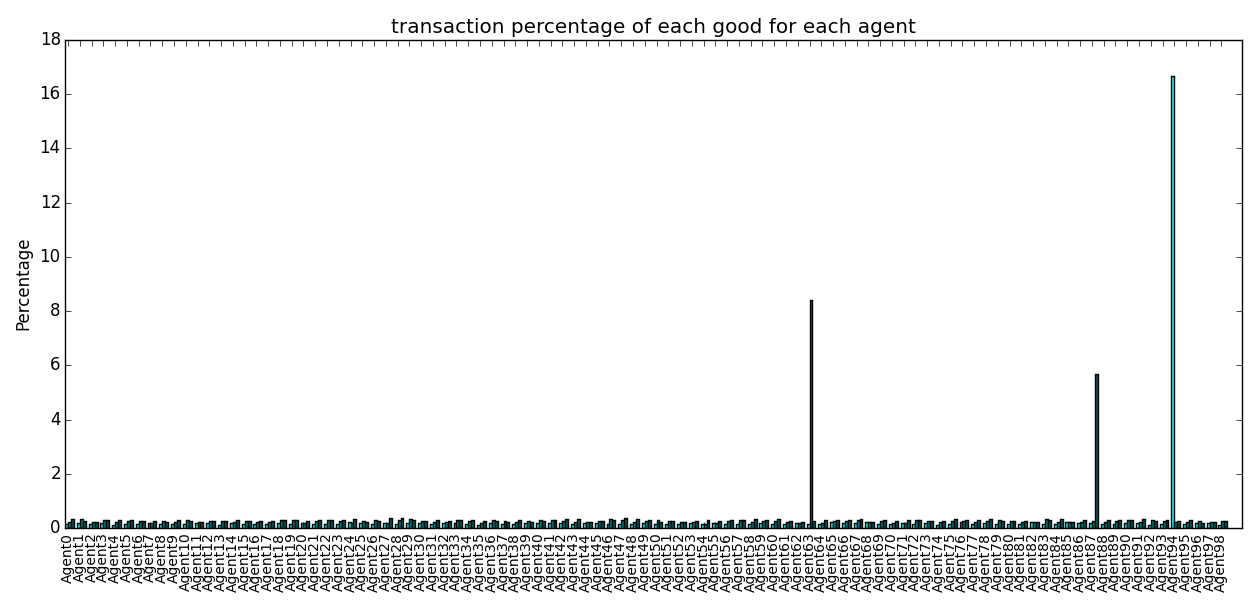
\includegraphics[scale=0.4]{experiment_images/RR_P}

\section{Balance rule}
The scenarios mentioned in the previous chapter are used in the simulator. To see if the number of goods used affects the results multiple experiments have been performed for every scenario, except for the basic scenarios, with a different amount of goods. Changing the amount of goods did not affect the results.
\subsection{Results}

\subsubsection{BS\_S}
Every time an agent receives a good the good is given back to the agent who gave the good. The moment P gives Q the good Q has the highest balance with P, because Q has received more from P than Q has given to P. This means that Q will give the good to P during the next transaction which means that all agents have the same balance with P again. Now P has to choose randomly who should receive the good next. No community arises, but the simulation is partially stabilized. It is partially stabilized because P will always get the good back after P has given it away. The only thing that is still random is the choice for P to who P should give to. \\
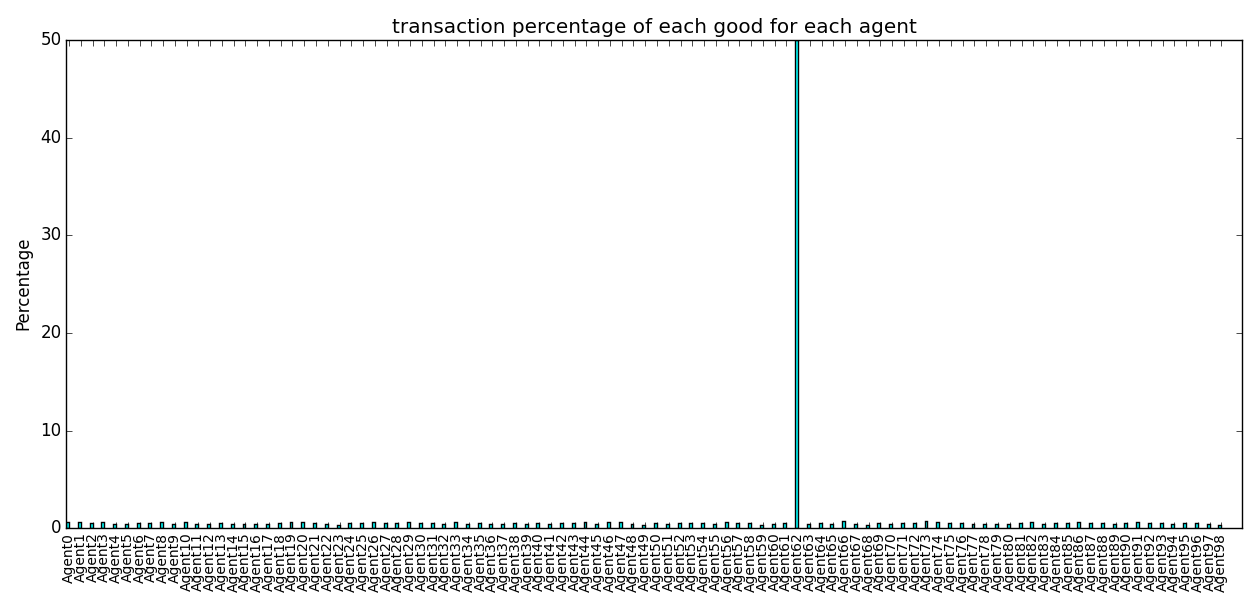
\includegraphics[scale=0.4]{experiment_images/BR_BS_S}

\subsubsection{BS\_P}
The producer participated in 50 percent of the transactions, because after each time the producer give away its product it perishes. Each other agent participated in approximately 0.5 percent of the transactions. The moment the producer gives the good to let's say agent Q the balance of the producer with Q is now lower then the balance of the producer with all other agents. This means that the next transaction the producer will not give to Q but has to choose randomly between all the other 98 agents, because the balance of the producer with the other agents is equal to each other. The same happens after the next transactions, now the producer has to choose randomly between 97 agents. This goes on untill 1 agent is left to choose from, at this point the choice is not random anymore, because only 1 agent is left. After this agent has received a good from the producer everyone is equal again and the whole process starts from the beginning. This leads to the conclusion that after every 98 transactions the next transaction can be predicted.  No community effect arisis, but the transactions are partially stabilized. \\
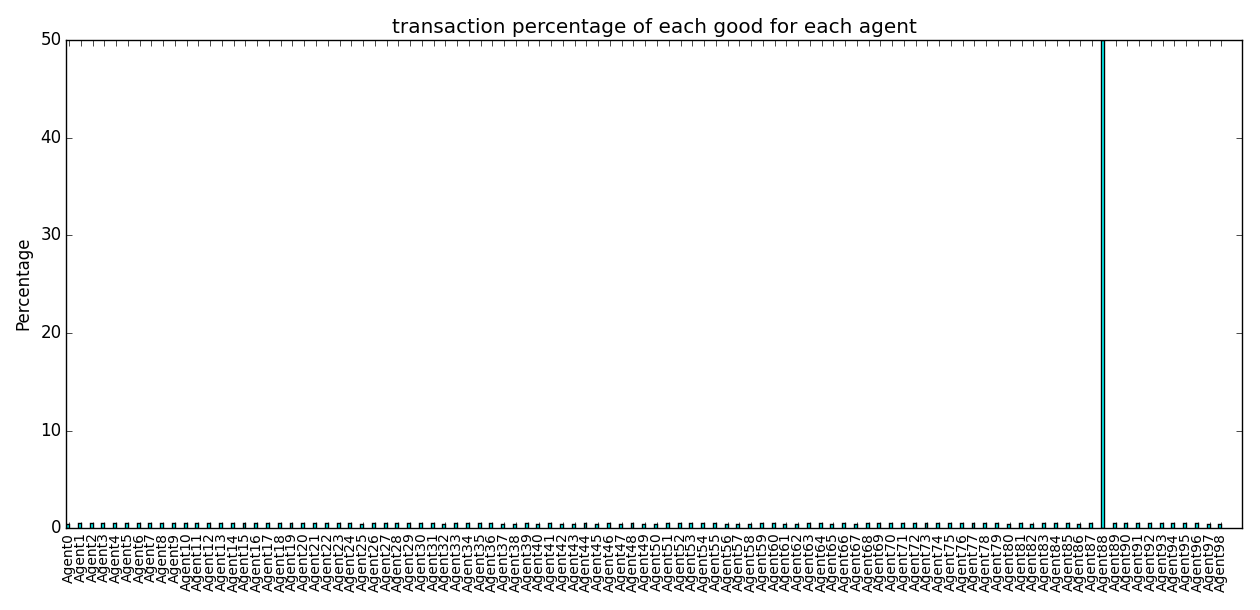
\includegraphics[scale=0.4]{experiment_images/BR_BS_P}

\subsubsection{BR\_S}
As expected the results are similar to the results from BS\_S where the goods are returned to the giving agent after each transaction. The only difference is is that the agents who start with the goods at the start of the simulation participate in proportion more in transactions of each others goods than the other agents do. This happens when two agents who start with the goods give to each other their good (they trade their good for the good of the other). When this happens they are able to give each others good to different agents. The following figure shows this situtuation. \\
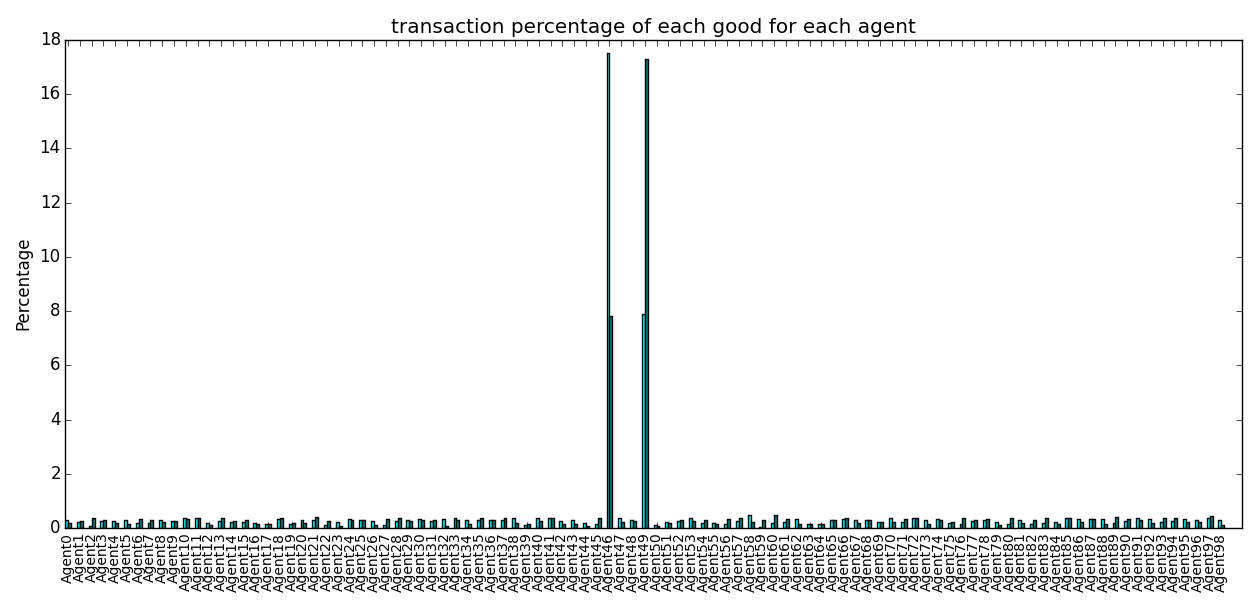
\includegraphics[scale=0.4]{experiment_images/BR_S}


\subsubsection{BR\_P}


\section{Goodwill rule}
All the scenarios mentioned in the previous chapter have been tested. The scenarios for the goodwill rule are split into two parts. The first part uses an account balance for the agents that start at 0. The second part uses an account balance for the agents that is randomly chosen and different for some agents at the start of the simulation. For every scenario except for the basic scenarios multiple experiment have been performed using a different amount of goods. The amount of goods used for each scenario are 1, 2, 5, 20, 50, 99.
\subsection{Results}

\subsubsection{BS\_S}
Immidiatly at the start of the simulation a community effect arises with a subgroup of size two. These subgroups only consists of agents with a like factor -1 or -0.5. The moment agent P gives to agent Q, Q is in debt with P. This means that Q values the next transaction more with P. So Q will give to P during the next transaction. Now P values the transaction with Q more than with any other agent, so P gives back to Q. An equilibrium has emerged where the yield of the transactions for P with Q an Q with P will switch between the same two values. The following yield curve shows what happens. 

\subsubsection{BS\_P}
The yield will approach zero, but it will never reach zero, because of the way the yield is calculated which is explained in chapter 2.2. No community effect arisis, but the transactions are partially stabilized. This is stabalization arises because the good perishes after the first time it is given by the producer. So all the agents will keep getting a good, but will never be able to give it away. Once an agent has received a good the yield for the producer with this agent is lower than the others. So the producer will randomly choose between the remaining agents who the producer has the same yield with. A same situation as with the BS\_P of the balance rule arisises where every 98 transactions are random and the 99th transaction is predictable.
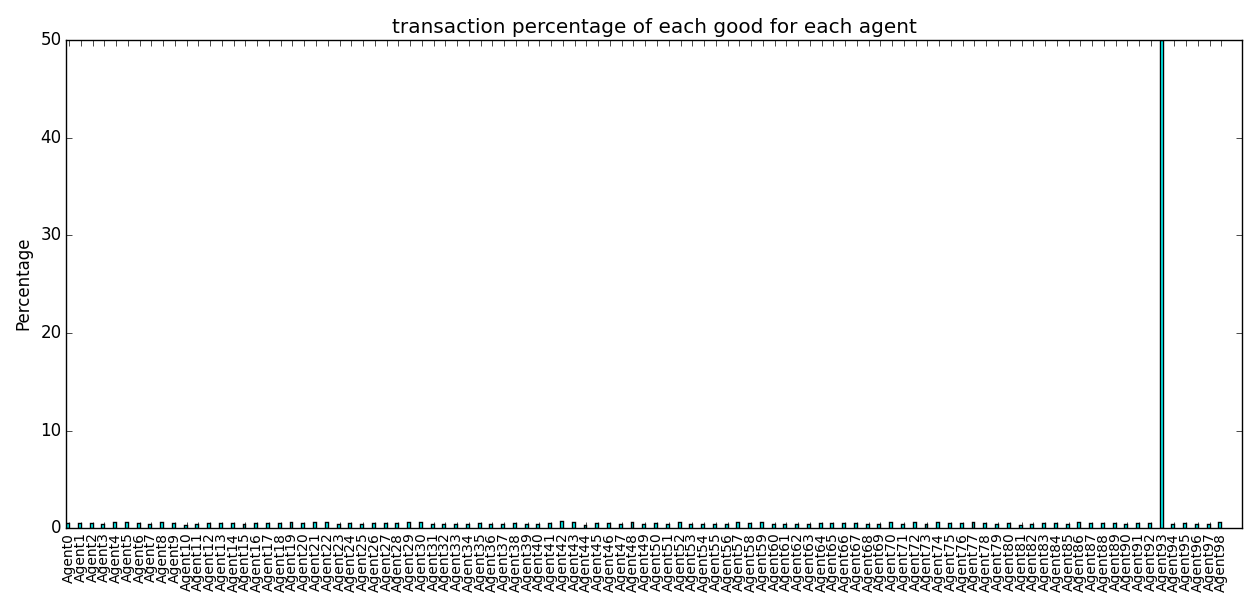
\includegraphics[scale=0.4]{GR_BS_P/4000transactions}

\subsubsection{GR\_L1B1N1}
Because all the balances are zero at the start and the nominal values are the same for every agent the yield of the first transaction is the same for everyone. The agent who first start with the good randomly gives the good to another agent. From this point on the subgroup has emerged and the good will only be traded between two agents. Good\_0 is from the beginning only traded within a subgroup of size 2.  When P gives to Q, Q is in debt with P and values giving to P more than giving to anyone else, the yield is the highest between Q and P. Q gives back to P and now the yield for P has become greater than the nominal value so P values the transaction with Q the most. An equilibrium just like with BS\_S has emerged. Changing the amount of goods did not change the results. Each good is only traded between 2 agents with a like factor of -1 or -0.5.

When perishable goods are used with a perish period of 1 the same as behaviour is shows as with BS\_P. When a higher perish period is used the goods act more like sustainable goods. 


\subsubsection{GR\_L1B1N2}
In the beginning some goods are traded between different agents. This happens because after some transactions the yield is the same value as the nominal value of the good. This means that the yield is the same for some agents. The agent who is giving the good will have to choose randomly between these agents, which can lead to a transaction with a different agent. This happens for example between agents where their nominal value is a multiple of the other and the like factors are -1 and -0.5. After a few transactions the calculation of the yield with these values results in the same value as the nominal value of the good, thus an agent needs to be randomly selected again. This is a rare occurance and eventually each good is only traded between 2 agents. Changing the amount of goods did not affect the results.
\subsubsection{GR\_L2B1N1}
The results are the same as the results from GR\_L1B1N1. Changing the size of the group with a like factor of -0.1 did not change anything. 
\subsubsection{GR\_L2B1N2}
The results are similar to the results from GR\_L1B1N2.  Changing the size of the group with a like factor of -0.1 did not change anything. 
\\
\\
The results above have shown that when the nominal values are the same and the account balance start at 0 for every agent that a subgroup (almost always) immediatly arises after the first transaction. Changing the nominal values so that the agents perceive them differently led to a more vivid environment where more agents participate in the transactions, but only occured under certain conditions which are not representative for a real life situation. 
\\
\\
further experiments will use different account balances at the start of the simulation.

\subsubsection{GR\_L1B2N1}
The first thing that the experiments with sustainable goods show is that in the beginning the transactions are mostly divided over the agents with a likefactor of -1 and -0.5. After the first 1000 transactions the transaction percentage is as follows. \\
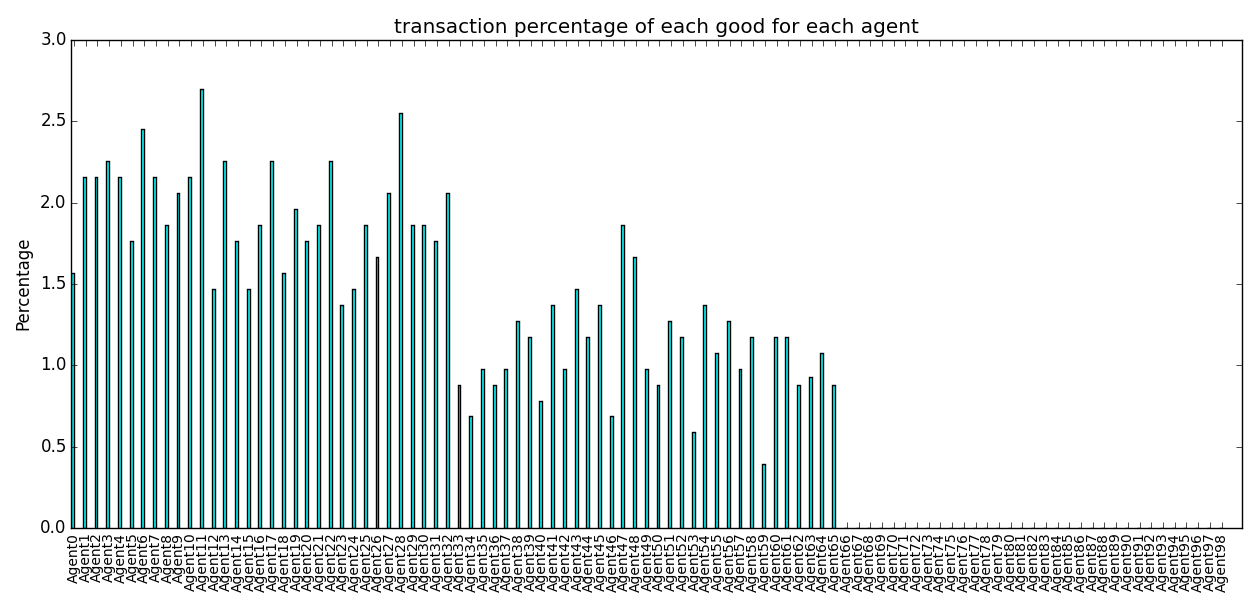
\includegraphics[scale=0.4]{GR_L1B2N1/1000transactions} \\
After 4000 transactions the subgroup started to arise. The figure below shows the emergence of this subgroup and show that the agents with a like factor of -0.1 eventually also participate in some transactions. \\
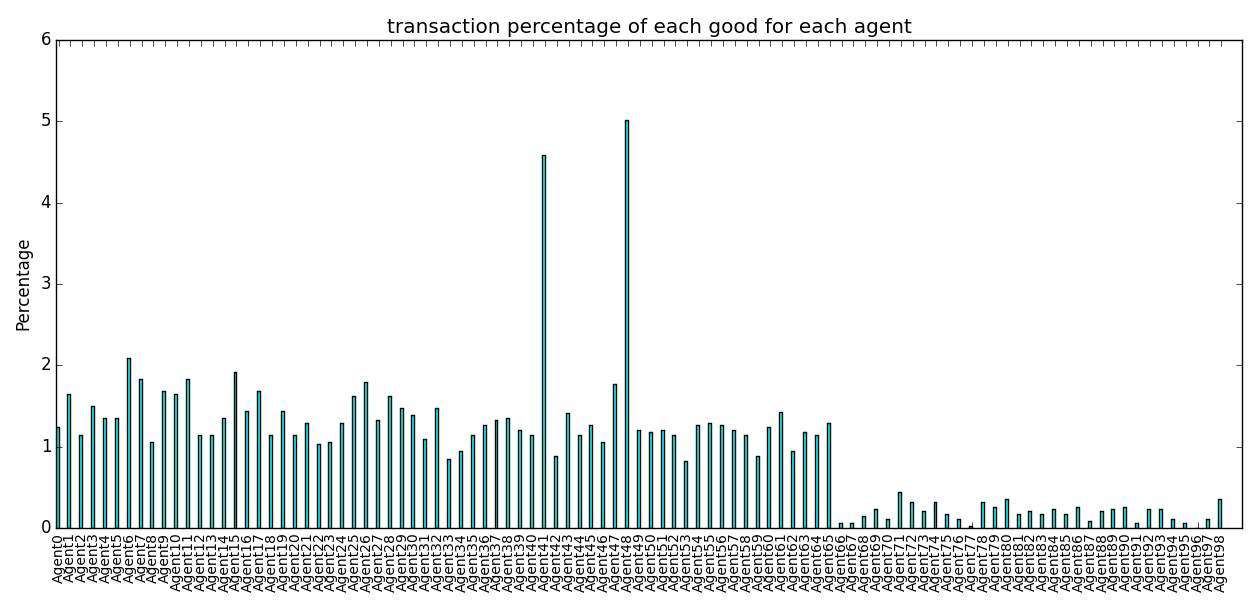
\includegraphics[scale=0.4]{GR_L1B2N1/3-5ktransactions1good} \\
 Every experiment with just one good led to a subgroup of agents with likefactor -0.5 or -1. With just one good the good was only traded between 2 agents after 4000-5000 transactions. When more goods are used the results start to vary alot more. The following figure shows what happens when more than one good is used. \\
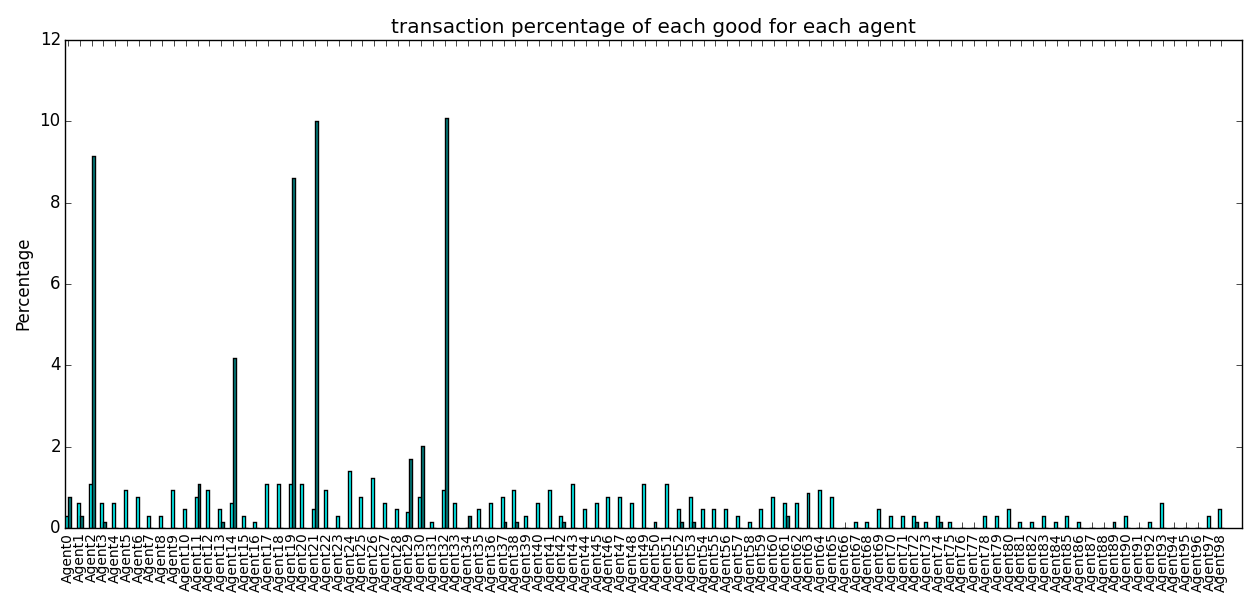
\includegraphics[scale=0.4]{GR_L1B2N1/3-5k_2goods_largergroups}
When more goods are used the goods sometimes fall into a subgroup for a short period of time. Eventually all goods are only traded between two agents. This same behaviour occurs when more goods are used. The goods are traded between multiple different subgroups untill the highest equilibrium arises where the yield switches between the two highest possible values. \\
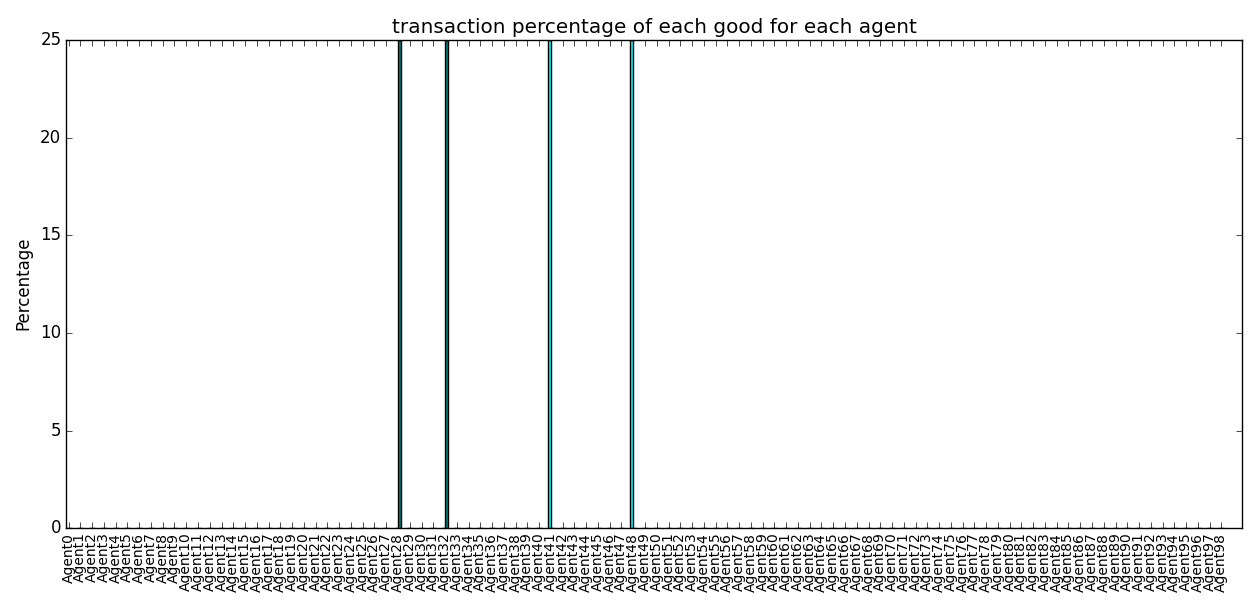
\includegraphics[scale=0.4]{GR_L1B2N1/10k_2goods_2subgroups}
The communities that arise only consists of agents with a like factor of -0.5 or -1. The more goods that are used the longer it takes before all goods are traded within a subgroup.

For the perishable goods the results are slightly different. With one perishable good and a perish period of 1 all experiments led to a community of the producer and all the agents with a like factor of -0.1 and -0.5. Because the good perishes after it has been given away by the producer the agents who receive the good stay in debt with the producer. The producer therefore prefers the agents with a like factor of -0.1 and -0.5 over -1. \\
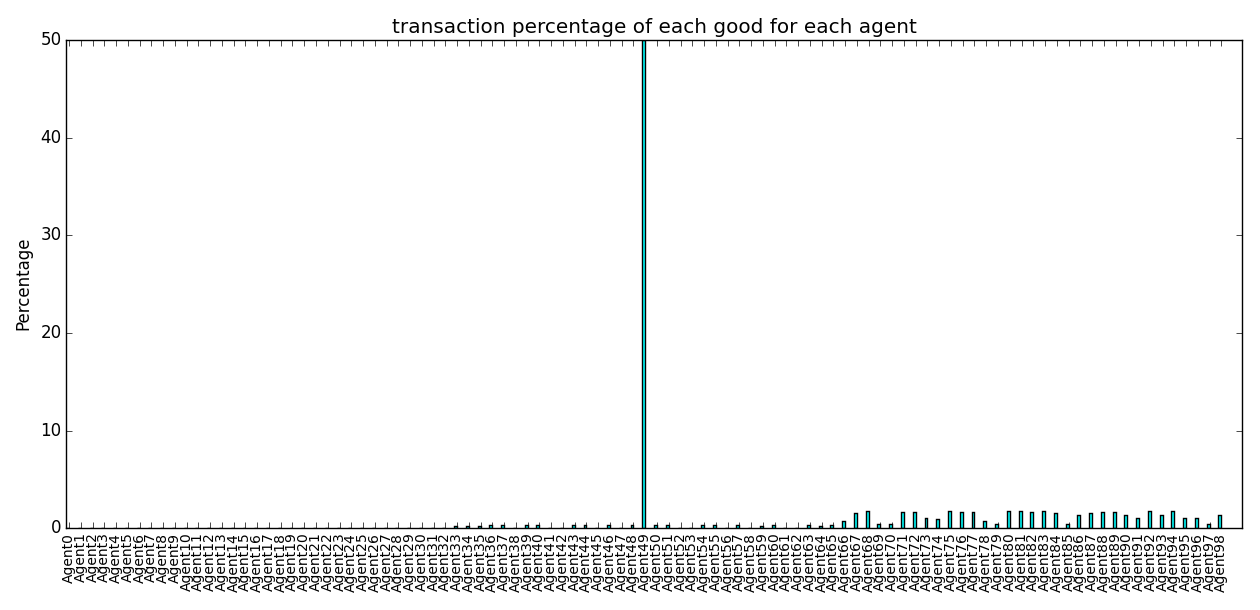
\includegraphics[scale=0.4]{GR_L1B2N1/1000transactions1perishable1-1} \\
When the perish period is higher than 1 the goods behave more like a sustainable good. The higher the perish period and the more perishable goods are used the longer it takes before a community arises.\\
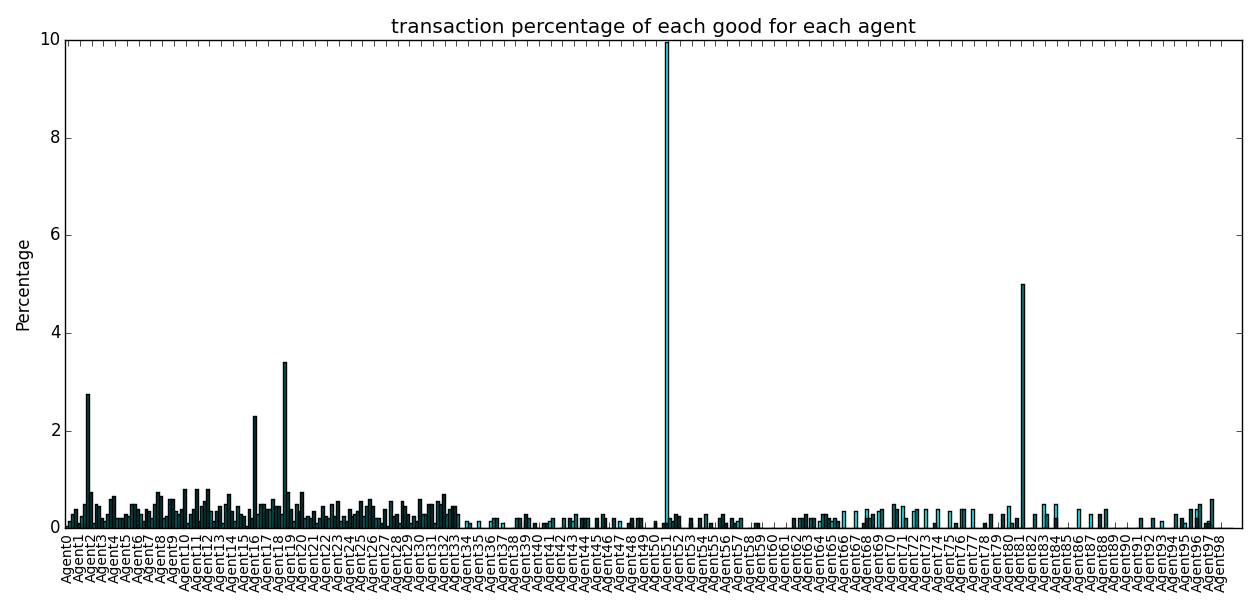
\includegraphics[scale=0.4]{GR_L1B2N1/1000transactions5perishable} \\
The figure above shows the distribution of the transactions of 5 perishable goods where good\_0 has a perish period of 1 and a production delay of 1, good\_1 has a perish period of 2 and a production delay of 2 etc. These results are after 1000 transactions and show that when the perish period gets higher (the darker green colored bars) the behaviour is more like a sustainable good. Eventually all goods are only traded within a subgroup of two agents, even when the perish period is 1.\textbf{ For the ... transactions the good with a perish period of 1 behaves as shown in figure .... But when more goods are used the producer of the good with a perish period of 1, for example agent P, sometimes gives his good to a producer, for example agent Q, who produce a good with a higher perish period. When this happens agent Q is in debt with P, but cannot give P's good back because it has perished. Q therefore has to give his own good to P. An equilibrium arise where both agents trade each others goods with each other.}\\
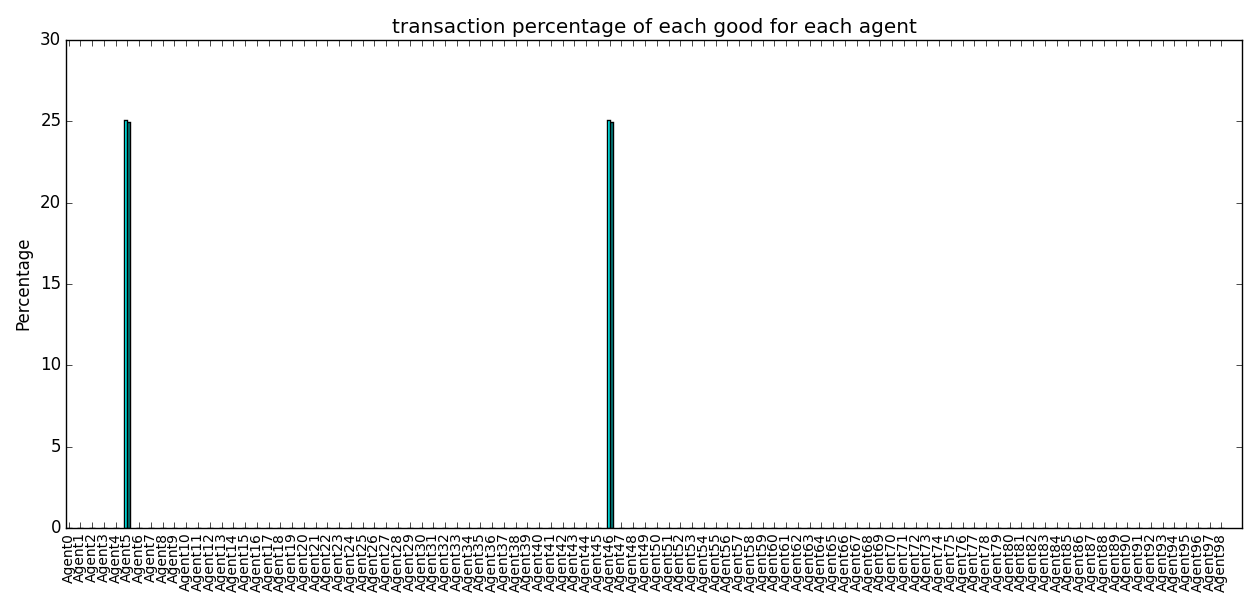
\includegraphics[scale=0.4]{GR_L1B2N1/2k_2perishable}


\subsubsection{GR\_L1B2N2}
With these experiments the nominal values are perceived differently by some agents. For the sustainable goods the results show that a community arises more quickly in comparison with GR\_L1B2N1 where the nominal values are the same for every agent. Where it took GR\_L1B2N1 with one good 4000-5000 transactions before a community arose these experiments only took 2000 transactions for one good. The distribution of the transactions in the beginning of the simulation is the same as with GR\_L1B2N1. Using more goods led to the same results, where all goods were only traded between two agents. If N2 would be changed so that the -1 like factor group perceives the nominal values of the goods higher than the -0.1 group then nothing changes to the results.
\\
For the perishable goods the results are the same as GR\_L1B2N1, but for this scenario the subgroups also arise more quickly.
\subsubsection{GR\_L2B2N1}
With this scenario only 5 agents have a like factor of -0.1 and the other agents have either -1 or -0.5. The major difference between this scenario and GR\_L1B2N1 is that the agents with a like factor of -0.1 are ignored more. The reason for this is simply, because the group with a like factor of -0.1 is smaller.
\subsubsection{GR\_L2B2N2}
The results are the same as GR\_L1B2N2. Changing the amount of agents with a like factor of -0.1 did not change anything.
\\
\\
The results of the goodwill scenarios show that what was expected did not happen. Instead of subgroups consisting of agents with a like factor of -0.1 the subgroups consist of agents with like factor -1 or -0.5. Instead of giving to agents who are liked more the agents in these scenarios prefer to give to agent who are not liked at all. On one hand this seems logical if you think about loans and in this case hostile loans where each time a good is given it leads to a high debt. With the yield curve used for this model receiving a good from someone who is not liked leads to a higher debt than receiving from someone who is liked, because the slope is heigher with a like factor of -1.On the other hand this seems illogical for a giving environment, where people rather give/pay of their debt with someone they like than with someone they don't like. This has led to a reconsideration of the yield curve used in this model.

\section{Reconsideration of the yield curve}
The results from the goodwill rule have revealed a problem. The problem is as follows: We have an agent P who is in possesion of a good and two other agents Q and R who P can give his good to. P has an account balance of 0 with both agents, P has a like factor of -0.1 with Q and a like factor of -1 with R. This would lead to the yield curve shown in figure .... \\
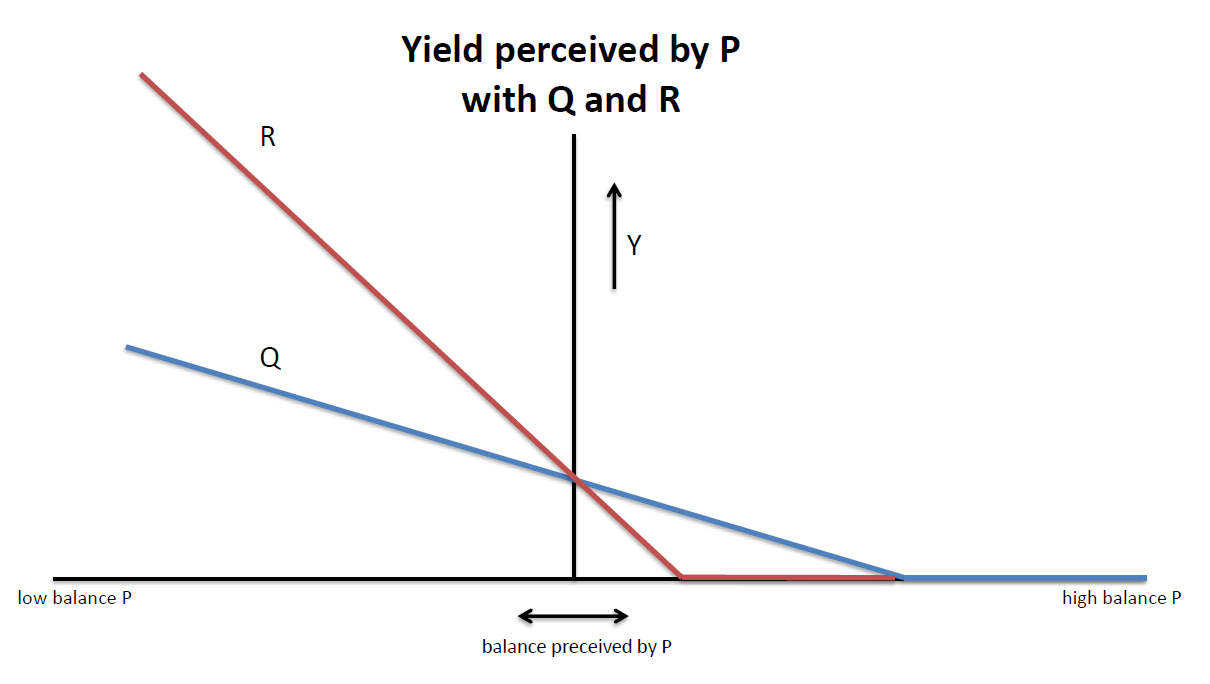
\includegraphics[scale=0.4]{YieldCurves/yieldcurve_P_QR}
\\
P now has to decide to who he will give the good. It would be logically to assume that because P likes Q more he will give to Q.The yield curve is currently defined as that the yield determines the choice to who the good will be given to. When the yield is the same for multiple agents an agent will be randomly selected. Accoriding to the yield it does not matter who is chosen, because all transactions are valued the same. So P will randomly choose between Q and R. Due to the results from the goodwill rule where the transactions are in favor of the lesser liked agents it has become clear that the way an agent is chosen when the yield is the same is not completly representative for a giving environment.

A solution to this problem would be to base the perception of the nominal value of a good on the like factors between all agent pairs. This would mean that for every good a NxN matrix needs to be created where the perception of the nominal value is different for every agent pair. However this solution requires alot of additional input data which would need to be created and stored by the user. A better solution would be to rewrite the calulation of the yield so that we get a yield curve shown in figure ... even when only one good is used. \\
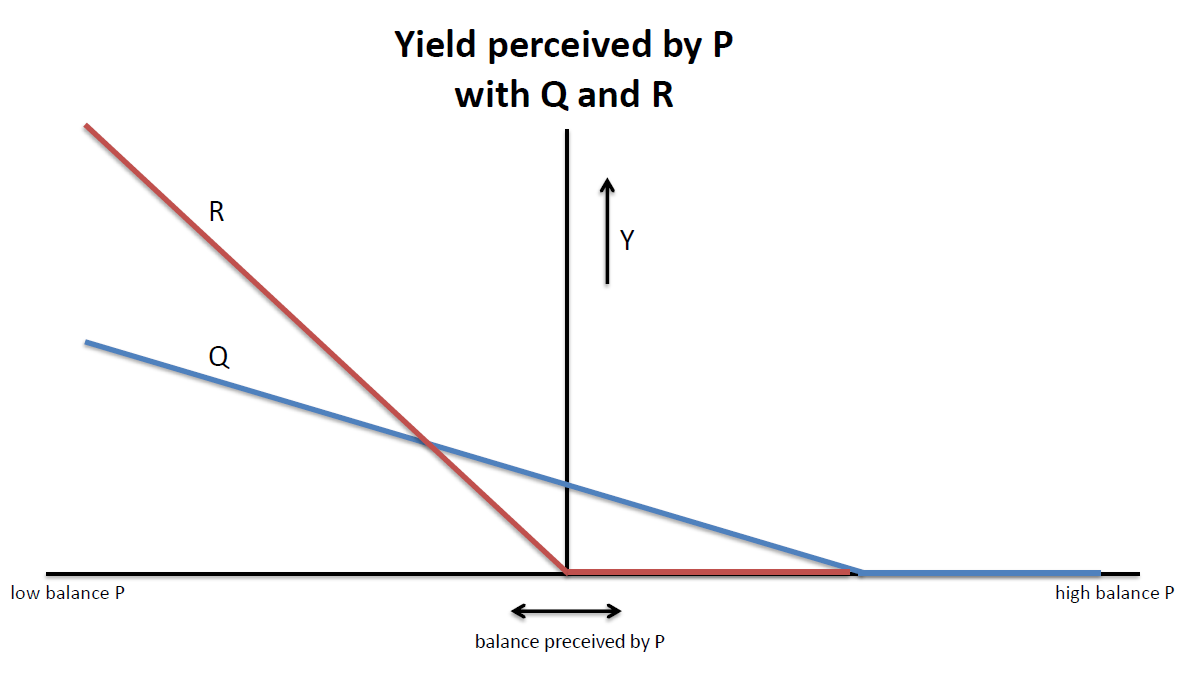
\includegraphics[scale=0.4]{YieldCurves/yieldcurve_P_QR2}

The yield curve in figure ... shows that with an account balance of 0 and a like factor of -1 the value of the transaction is lower than when the like factor would be -0.1. In this case P would choose Q over R, because a transaction with a 'friend' is worth more than with a stranger. This means that when the nominal value is defined as a constant than the intercept(\textit{b}) in \textit{$Y = aX + b$} should be a lower value when the like factor is also lower. To accomplish this we can assume that \textit{b} will scale equally with the like factor, thus \textit{$Y = aX + b(1 + a)$}.  The calculation of the yield needs to be rewritten as follows:
\begin{equation}
\begin{split}
  Y & = aX + b \\
     & = aX + b(1 + a) \\
     & = aX + b + ab \\
     & = a(X + b) + b 
\end{split}
\end{equation}
This new calculation of the yield leads to yield curves just like the one in figure ... and solves the problem of choosing an agent when the balance is 0. To see what the effect is of these changes on the results of the goodwill scenarios additional experiments have been performed with the revised yield curve. The results of the experiments that show major differences in results are explained below.

\begin{description}
\item[GR\_L1B1N1] In comparison to the previous experiment the subgroups don't emerge immedieatly after the first transactions. The transactions are distributed as shown in figure ... until a community arises. It takes on average 10000 transacitons before every good is eventually traded within a subgroup of two agents. These communities only exist within the agents with a like factor of -0.1. Changing the amount of goods does not affect the results. \\
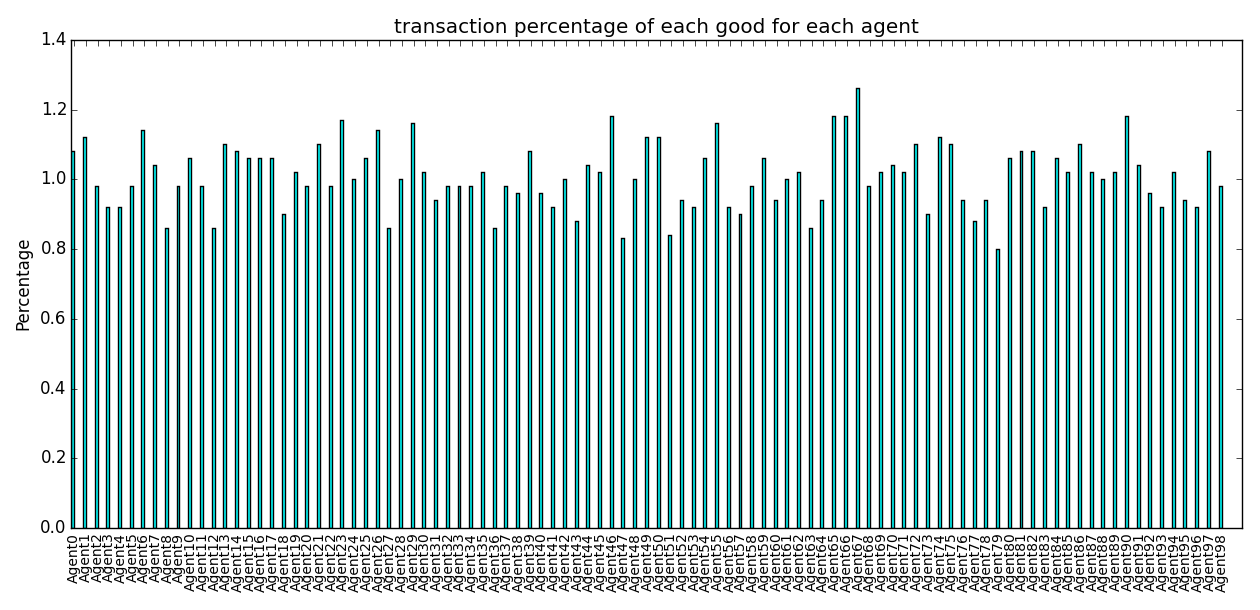
\includegraphics[scale=0.4]{GR_L1B2N1/5k_1good_b1n1}

\item[GR\_L1B1N2] When N2 is used where the nominal values are perceived higher by the agent with a -0.1 like factor than the agents with a -1 like factor then the disitribution is as shown in figure ... Eventually every good is only traded between two agents.. \\
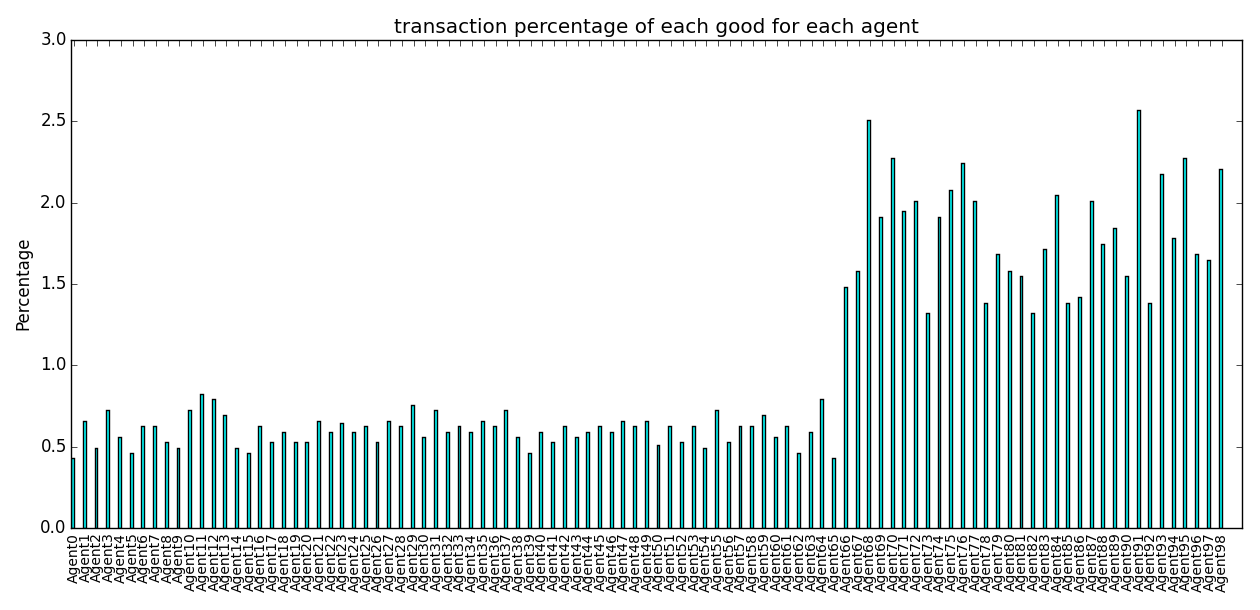
\includegraphics[scale=0.4]{GR_L1B2N2/3k_1good_b1n2} 

If N2 would be changed so that the agent with a -1 like factor perceive the nominal values of the goods higher than the agent with a -0.1 like factor then the transactions would in the beginning be in favour of the agents with a like factor of -1 and lead to the distribution shown in figure ...  \\
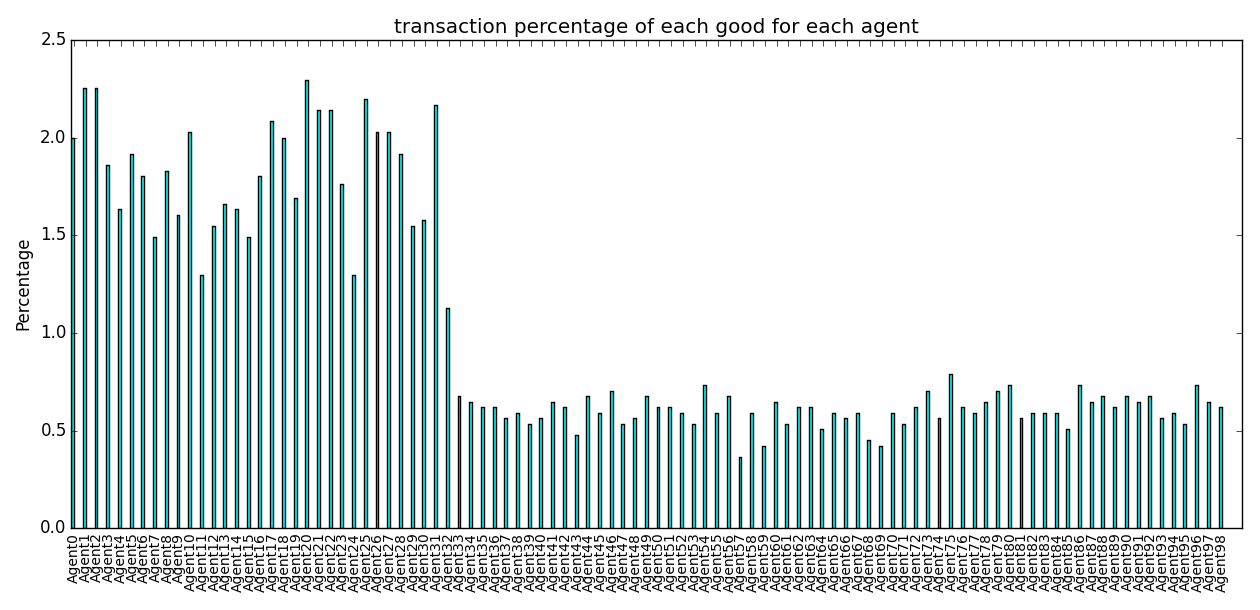
\includegraphics[scale=0.4]{GR_L1B2N2/3k_1good_b1n3} \\
Eventually a subgroup arisis as shown in figure ... The transactions within this subgroup do not stabilize, because the transactions are still random within this subgroup. This randomness occurs, because within these communities the yield sometimes reaches the same value for multiple agents. For example when an agent has to choose between two agents who have the same like factor and the balance with these two agents is the same the choice will still be random.\\
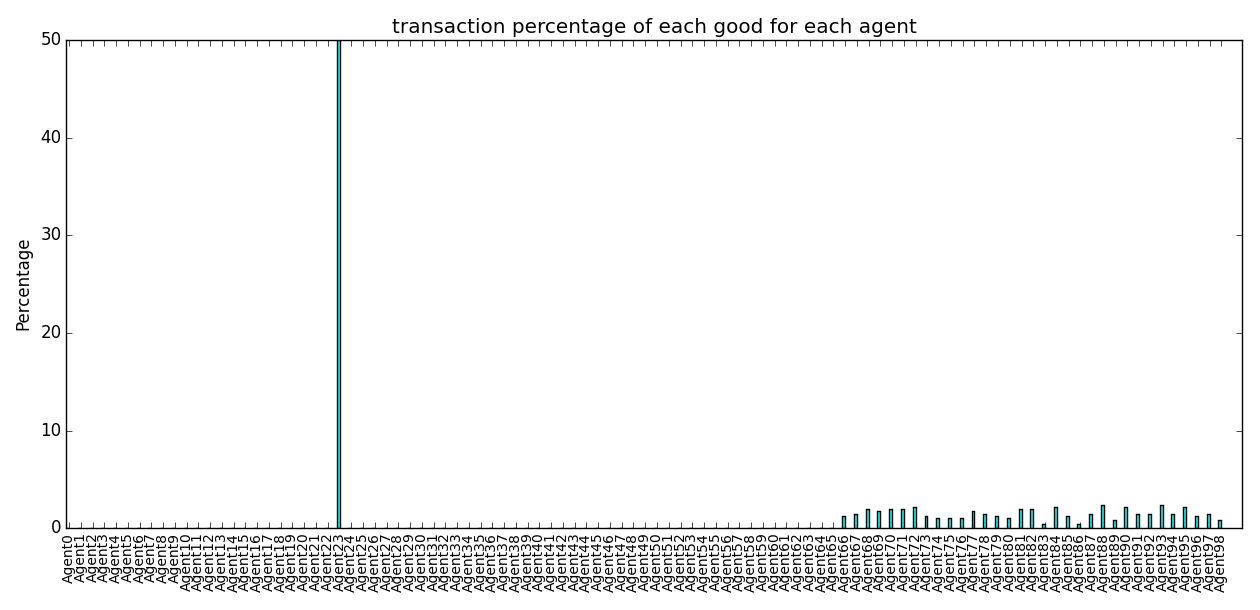
\includegraphics[scale=0.4]{GR_L1B2N2/5k_1good_b1n3subgroup}
\end{description}
The major difference between the revised yield curve and the original one is that when B1 is used a community does not immediatly arise. The transactions are also more evenly distributed at the start and eventually are in favour of the agents with a like factor of -0.1 as shown in figure .... and .... Also when the nominal values vary more then the transactions are in favour of the group who has the highest perception of the nominal values.
When B2 is used the results are simmilar to GR\_L1B1N2, but the distribution in the beginning is always just like in figure.... Eventually also with B2 every good is mostly traded  between two agents with a like factor of -0.1. In some cases the subgroup consists of 3-5 agents with the possibility of an agent with a like factor of -0.5 that joins the community. When L2 is used nothing changes to the results.

Just as the expactations were prior to the experiments, the agents prefer to give to agents who are liked and try to ignore the agents who are less liked.









\section{Goodwill rule 2.0}
All the scenarios mentioned in the previous chapter have been tested. The scenarios for the goodwill rule are split into two parts. The first part uses an account balance for the agents that start at 0. The second part uses an account balance for the agents that is randomly chosen and different for some agents at the start of the simulation. For every scenario except for the basic scenarios multiple experiment have been performed using a different amount of goods. The amount of goods used for each scenario are 1, 2, 5, 20, 50, 99.
\subsection{Results}

\subsubsection{BS\_S}
Immidiatly at the start of the simulation a community effect arises with a subgroup of size two. The moment agent P gives to agent Q, Q is in debt with P. This means that Q values the next transaction more with P. So Q will give to P during the next transaction. Now P values the transaction with Q more than with any other agent, so P gives back to Q. An equilibrium has emerged where the yield of the transactions for P with Q an Q with P will switch between the same two values. The following yield curve shows what happens. 

\subsubsection{BS\_P}
The yield will approach zero, but it will never reach zero, because of the way the yield is calculated which is explained in chapter 2.2. No community effect arisis, but the transactions are partially stabilized. This is stabalization arises because the good perishes after the first time it is given by the producer. So all the agents will keep getting a good, but will never be able to give it away. Once an agent has received a good the yield for the producer with this agent is lower than the others. So the producer will randomly choose between the remaining agents who the producer has the same yield with. A same situation as with the BS\_P of the balance rule arisises where every 98 transactions are random and the 99th transaction is predictable.
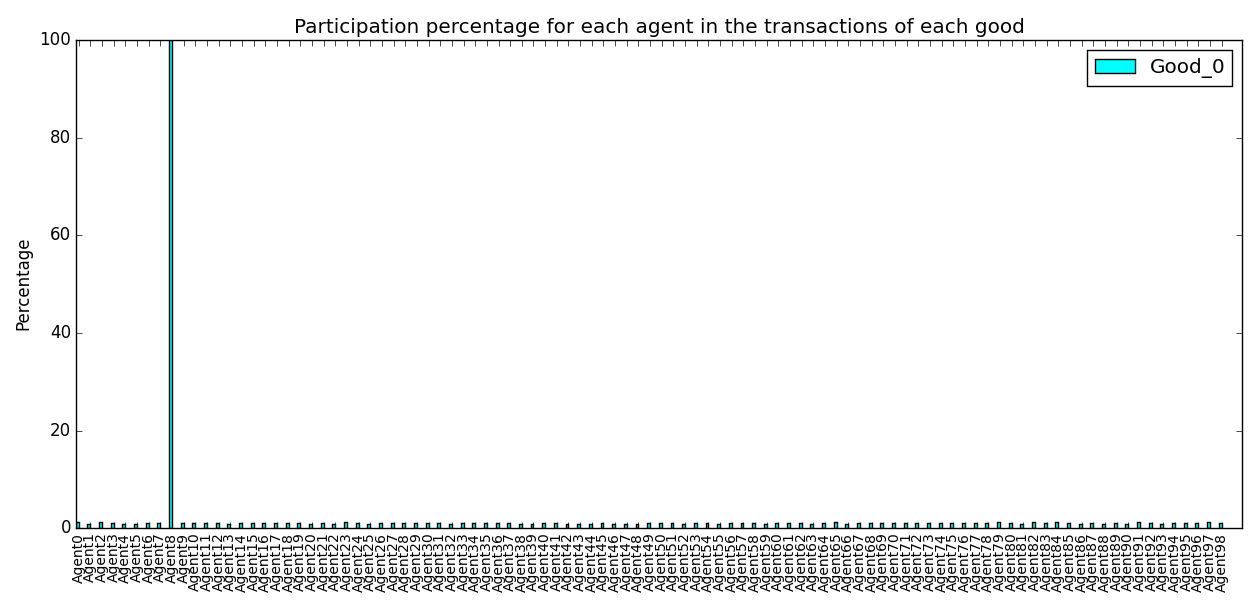
\includegraphics[scale=0.4]{Simulation_figures/GR_BS_P/Figure1_10k}

\subsubsection{GR\_L1B1N1}
When the good start at an agent with like factor -1 the good is gien away to a agent with like factor -0.1. Once the good is in possesion of an agent with like factor -0.1 a subgroup arises between two agents with a like factor -0.1. When the good start at an agent with like factor -0.5 the good is also given to an agent with like factor -0.1. This time a subgroup arisises between the agent with like factor -0.5 and the agent with like factor -0.1 who reived the good the first time. When more goods are used the results stay the same.

When perishable goods are used with a perish period of 1 the same as behaviour is shows as with BS\_P. \textbf{MORE RESULTS HERE}


\subsubsection{GR\_L1B1N2}
When N2 is used where the nominal values are perceived higher by the agent with a -0.1 like factor than the agents with a -1 like factor then the results are similar the the results from GR\_L1B1N1. The only difference is that the subgroups only consist of agent with a like factor of -0.1.
When more goods are used the results do not change.
If N2 would be changed so that the agent with a -1 like factor perceive the nominal values of the goods higher than the agent with a -0.1 like factor then the results are as shown in figure .... When the good starts at an agent with a like factor of -0.1 a subgroup immediatly arises where the good is only traded between two agents with a like factor of -0.1.
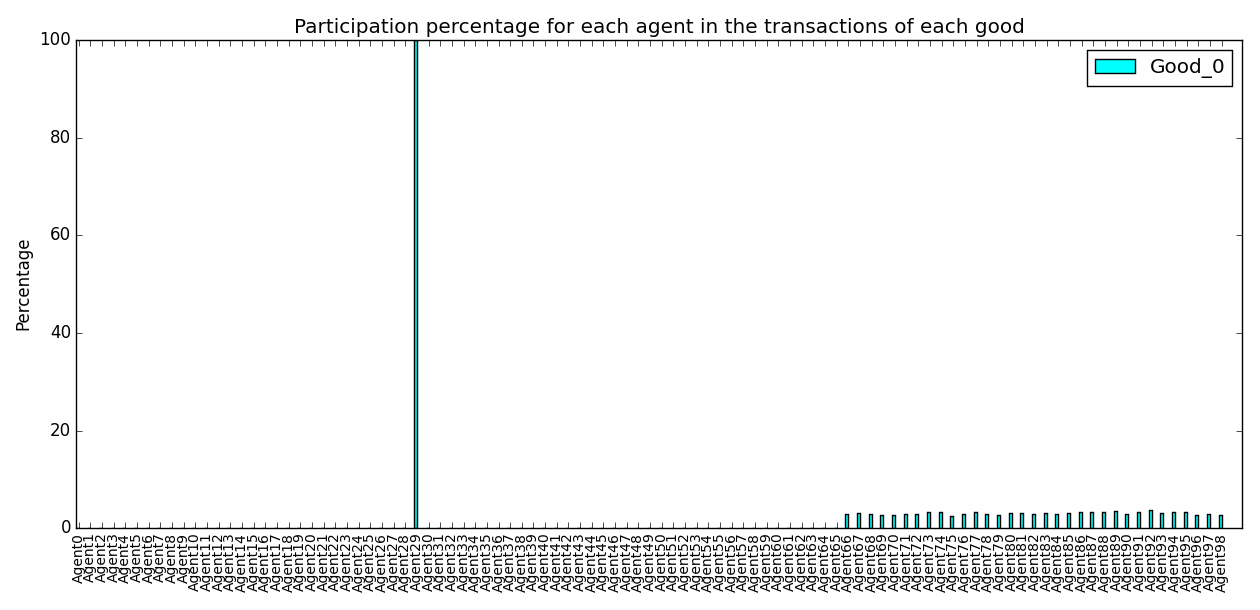
\includegraphics[scale=0.4]{Simulation_figures/GR_L1B1N2/321_1good}
When more goods are used and some goods start at agents with like factors -1 or -0.5 and other goods start at agents with like factors -0.1 then a subgroup shown in figure ... arises. The spikes shown in this figure in the group with like factor -0.1 (agent\_66-agent\_98) switch between different agents over time.

\subsubsection{GR\_L2B1N1}
The results are the same as the results from GR\_L1B1N1. Changing the size of the group with a like factor of -0.1 did not change anything. 
\subsubsection{GR\_L2B1N2}
The results are the same as the results from GR\_L1B1N1. Changing the size of the group with a like factor of -0.1 did not change anything. 

\subsubsection{GR\_L1B2N1}
After approximatly 100 transactions a subgroup consisting of two agents with like factors -0.1 arises. As shown in figure ... some transactions in the beginning take place between agents with a lower like factor. When more goods are used more transactions take place before a subgroup arises. For two goods the subgroup arises after approximatly 1000 transactions. Eventaully every good is only traded between two agents with like factors -0.1


\subsubsection{GR\_L1B2N2}

\subsubsection{GR\_L2B2N1}

\subsubsection{GR\_L2B2N2}



\textbf{PERISHABLE GOODS TESTEN}




\chapter{Conclusions and Discussions}
The created simulation program provides a wide range of possible sccenarios to simulate the giving game designed for this thesis. With the provided visualization of the behaviour during the giving game the results are promosing. 

The scenarios of the random rule and balance rule were very basic scenarios to test the implemented giving game. The behaviour of both the random rule and the balance rule was very predictable and showed a correct implementation of the giving game. The balance rule also confirmed a correct calculation of the community effect.

The first experiments of the goodwill rule showed suprising results. These results have led to a reconsideration of the yield curve which caused an improvement in the simulation model for the giving game. The results from the additional experiments confirmed the hypothesis, but these results  are still difficult to clarify with a real life scenario. It can be concluded that in most cases people rather give to 'friends' than to strangers. Some experiments showed a distribution of the transactions in favour of the less liked agents or a community where also an agent who is less liked was part of. These experiments are easily understood from a mathematical perspective, because the calculation yield can lead to an equilibrium between two different agents. But from a more psychological perspective it is difficult to understand why someone would still want to trade with someone who is not liked.\\
\\
Even though some of the experiments are difficult to explain with a real life scenario the research questions can still be answered.
\\
\\
\textit{In a Giving Game simulation will transactions eventually take place within a limited subgroup of the entire population?} \\
The answer to this question is simply, yes. All the experiments eventually led to subgroups of size 2 and when the nominal values were perceived differently by the agents the subgroups could consist of more than 2 agents. As expected in the first place the revised yield curve led to subgroups consisting mostly of agents who like each other.
\\
\\
\textit{In a Giving Game simulation will we see a repeating sequence of transactions or will the transaction sequence look random?} \\
The balance rule and the goodwill rule showed a partial stabilization of the transactions when a perishable good was used with a perish period of 1. All the other experiments did not lead to a repeating sequence of transactions. Even when communties larger than two agents arose the transactions within these communties were random.

\section{Further research}
Further experiments will allow the use of more variety in the parameters used for the goodwill rule. 

A possible variant on the giving game used in this thesis is that agents are able to hold on to a good. This is leads to a similar simulation as used in the article 'Money Network in Kiyotaki-Wright Model'. Holding on to a good is a more realistic approach, but comes with a few extra parameters. Realistically holding on to a good means that the good needs to be stored somewhere. In the real world this would mean that storage costs have to be paid and certain goods (perishable goods) would not be able to be stored forever. The time an agent holds on to a good is also a parameter that can influence the choice for the transaction.

\chapter{Appendix A}

\section{Simulator manual}

\section{Code Documentation}



\end{document}